For each signal, find the Fourier transform, $X(\omega)$, and then plot $|X(\omega)|$ 
(note, you may want to use MATLAB for the plot in 3.)

\section*{Problem 1}

\begin{figure}[H]
\caption*{}
\centering
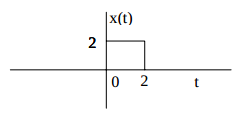
\includegraphics[width=0.4\textwidth]{figs/c2p11.png}
\label{fig:}
\end{figure} 

\subsection*{Solution}
Taking the derivative of $x(t)$ we get:

\begin{figure}[H]
\caption{Derivative $\dot{x}$}
\centering
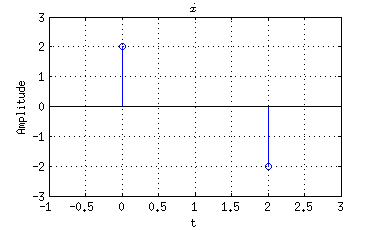
\includegraphics[width=0.6\textwidth]{figs/c2p1dotx.png}
\label{fig:}
\end{figure}

Applying \ref{eq:c21} and \ref{eq:c22c} to $\dot{x}$ we have:

\begin{equation*}
\begin{aligned}
j \omega X(\omega) &= 2 \int_{-\infty}^\infty (\delta(t) - \delta(t-2))e^{-j \omega t} \; dt\\
&= 2 [ 1 - e^{-2 j \omega}] \\
&= 2 e^{-j \omega}[ e^{- j \omega} - e^{- j \omega}] \\
&= 4 j e^{-j \omega} \sin(\omega) \\
X(\omega) &= 4 \frac{\sin(\omega) }{\omega} e^{-j \omega} \\
 &= 4 Sa(\omega) e^{- j \omega}
\end{aligned}
\end{equation*} 

The plot of the magintude and angle of $X(\omega)$ is:
\zcodemat{sources/c2p1a.m}{Plot of Magnitude and Angle}

\begin{figure}[H]
\caption{Magnitude $|X(\omega)|$ and Angle}
\centering
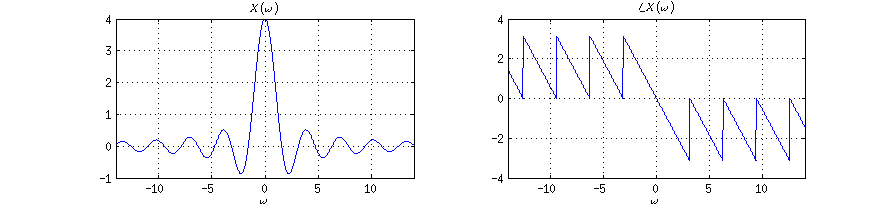
\includegraphics[width=1.0\textwidth]{figs/c2p1a.png}
\label{fig:c2p1a}
\end{figure} 

